\section{Simulation Analysis}

In this section we present the results obtained for a 10 period simulation of the circuit.

\subsection{Envelope Detector Output}

\begin{figure}[h] \centering
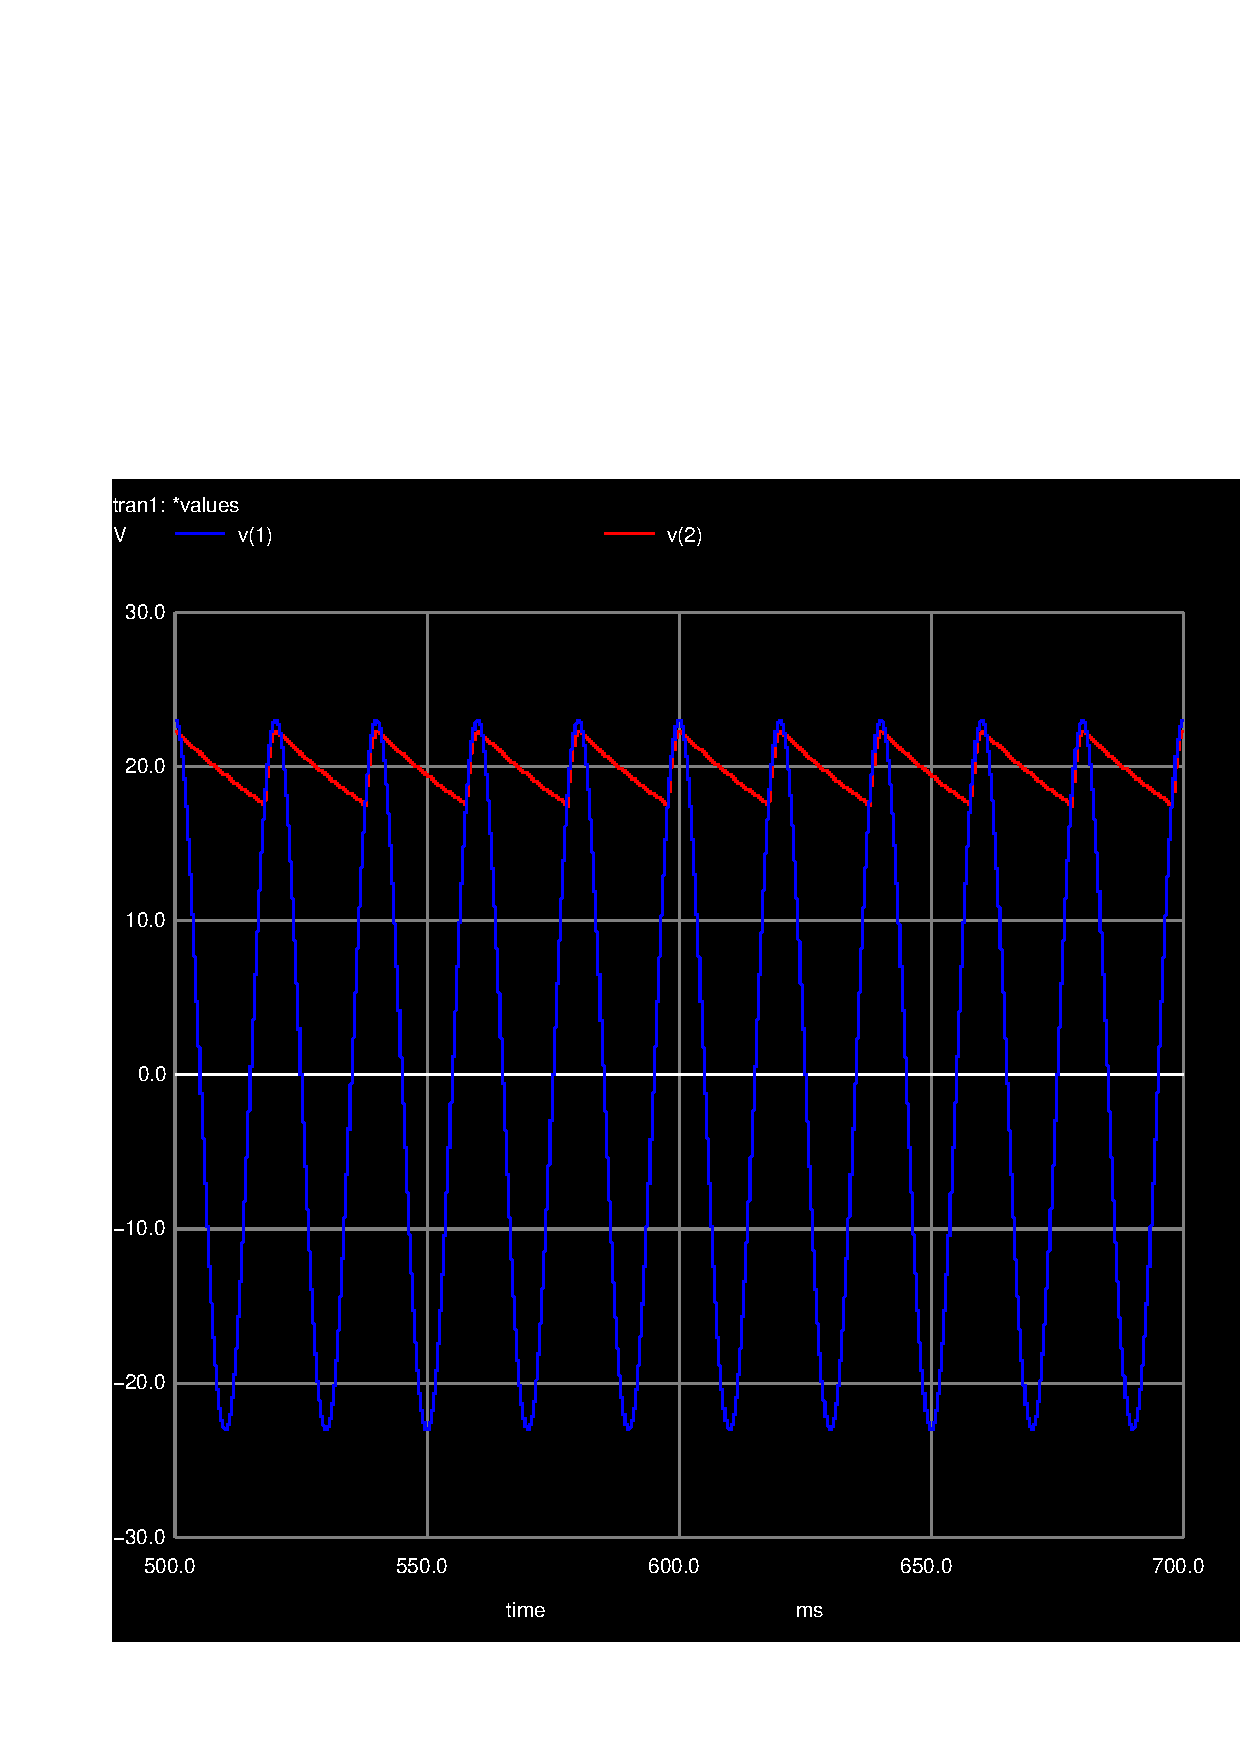
\includegraphics[width=0.6\linewidth]{ven.pdf}
\caption{vO Envelope Detector}
\label{fig:Ven}
\end{figure}

\begin{table}[h]
  \centering
  \begin{tabular}{|l|r|}
    \hline    
    {\bf Name} & {\bf Value [V]} \\ \hline
    \input{../sim/Envelopeng_tab}
  \end{tabular}
  \caption{Envelope Detector}
  \label{tab:Envelopeng}
\end{table}
\FloatBarrier

\subsection{Voltage Regulator Output}

\begin{figure}[h] \centering
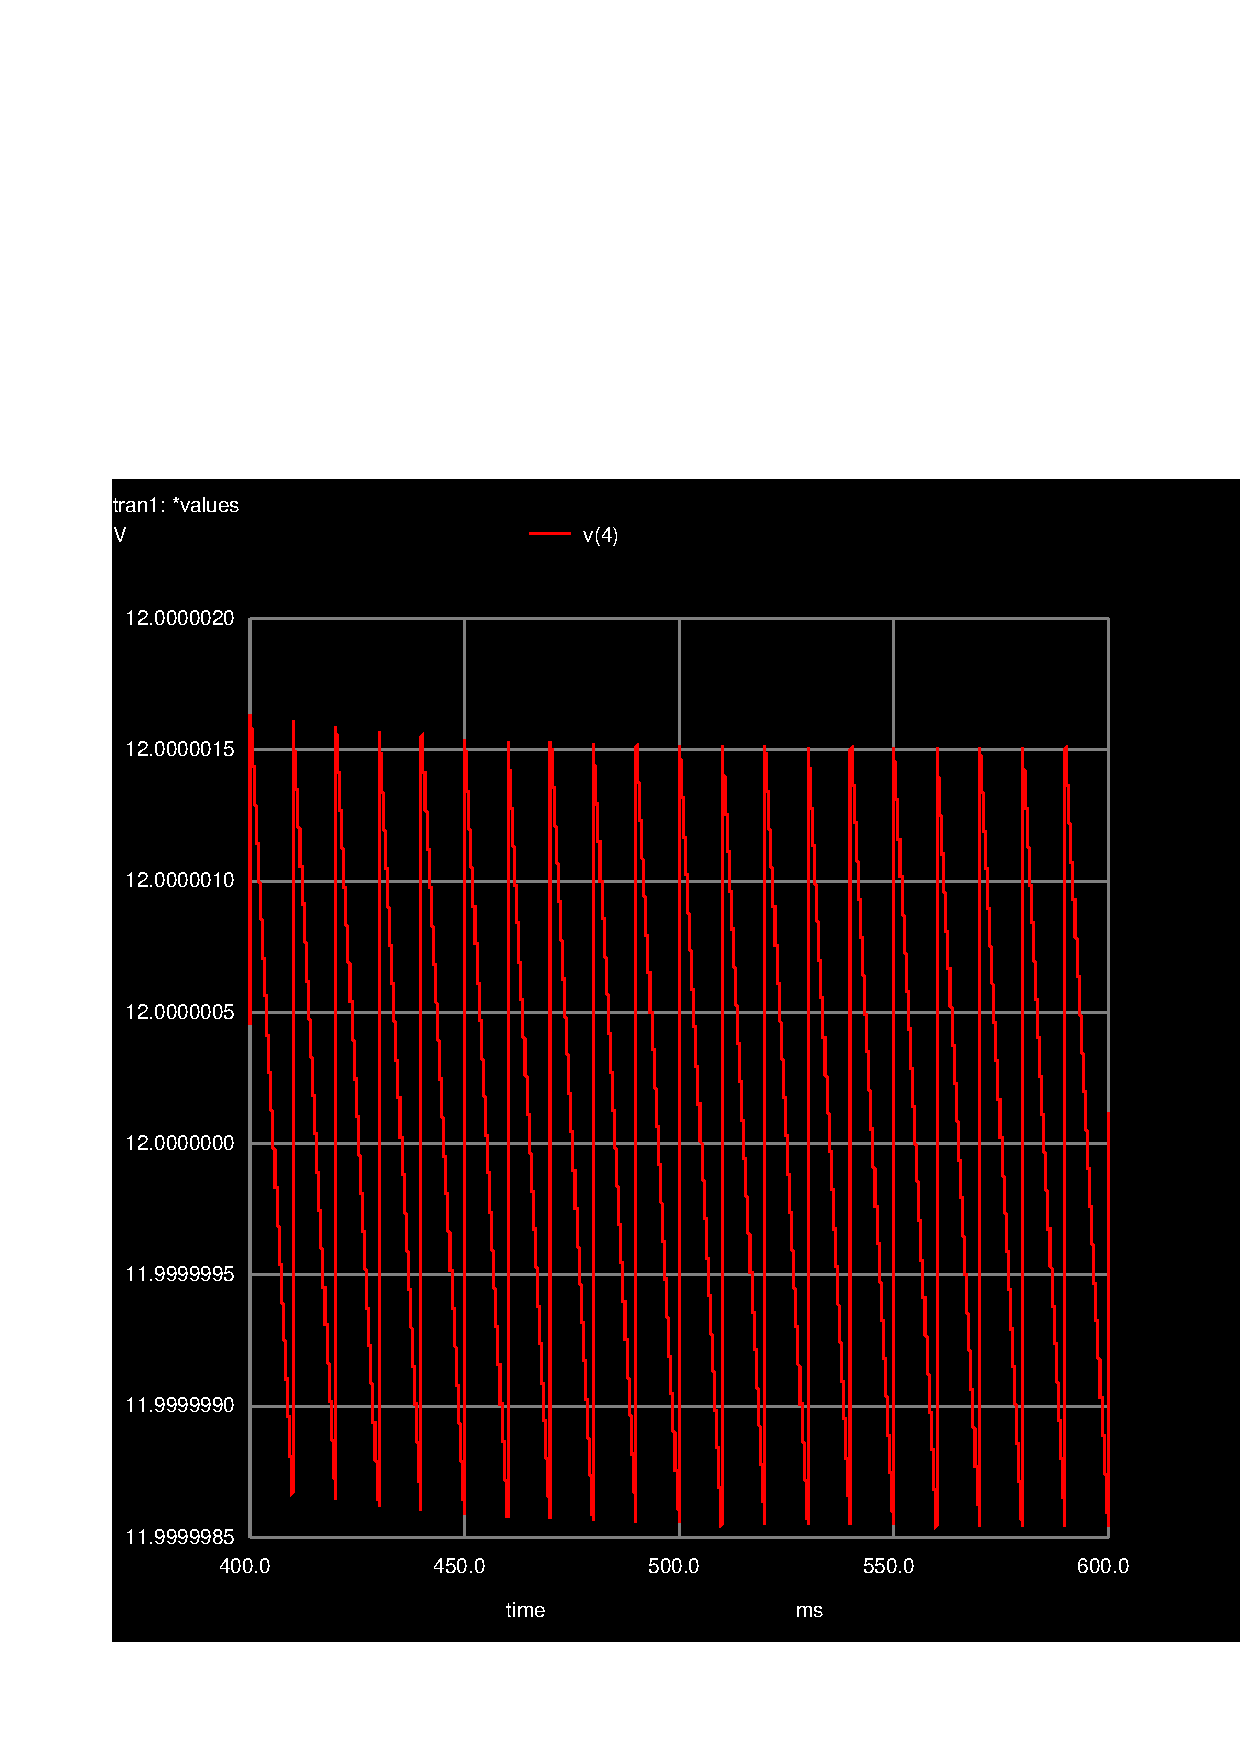
\includegraphics[width=0.6\linewidth]{vout.pdf}
\caption{vO Voltage Regulator}
\label{fig:vOregng}
\end{figure}


\begin{figure}[h] \centering
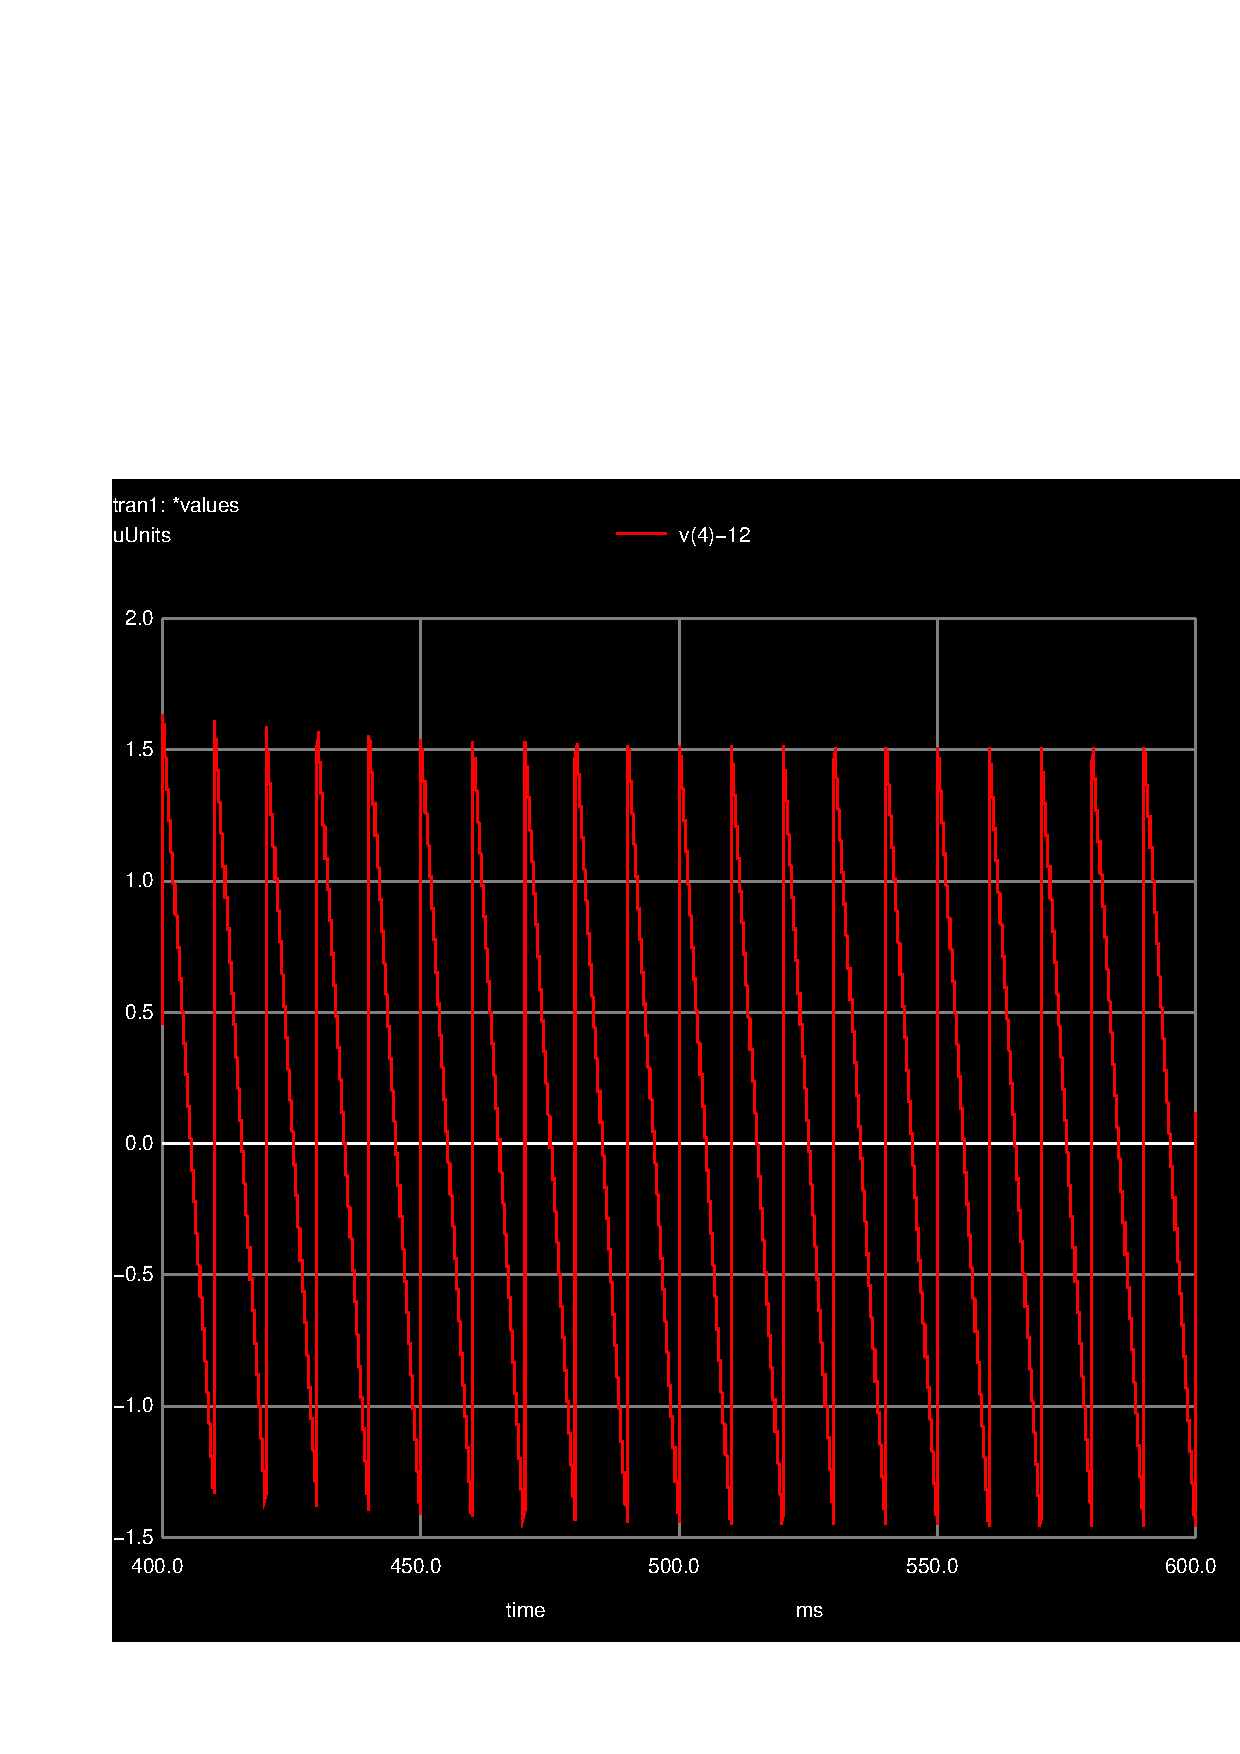
\includegraphics[width=0.6\linewidth]{vout-12.pdf}
\caption{vO Voltage Regulator - 12}
\label{fig:vO-12ng}
\end{figure}


\begin{table}[h]
  \centering
  \begin{tabular}{|l|r|}
    \hline    
    {\bf Name} & {\bf Value [V]} \\ \hline
    \input{../sim/Regulatorng_tab}
  \end{tabular}
  \caption{Voltage Regulator}
  \label{tab:Regulatorng}
\end{table}
\FloatBarrier

\subsection{Cost and Merit}

\begin{table}[h]
  \centering
  \begin{tabular}{|l|r|}
    \hline    
    {\bf Name} & {\bf Value [V]} \\ \hline
    \input{../sim/Meritng_tab}
  \end{tabular}
  \caption{Cost and Merit}
  \label{tab:Meritng}
\end{table}
\FloatBarrier

